\begin{exercice*} 
    Sur la figure ci-dessous :
    \begin{itemize}
        \item Les points $A$, $M$, $B$ sont alignés.
        \item Les points $A$, $N$, $C$ sont alignés.
    \end{itemize}
    \begin{tikzpicture}
        % \draw[help lines, color=black!30, dashed] (0,0) grid (9,5);                
        \coordinate (A) at (1,5);
        \tkzLabelPoints[above,xshift=-2mm,yshift=2mm](A);
        \coordinate (B) at (0,1);
        \tkzLabelPoints[left](B);                
        \coordinate (C) at (5,4);
        \tkzLabelPoints[right](C);
        \tkzDrawSegment(B,C);
        \tkzDefPointBy[homothety=center A ratio 0.6](C)	\tkzGetPoint{N};            
        \tkzLabelPoints[above right](N);
        \tkzDefPointBy[homothety=center A ratio 0.6](B)	\tkzGetPoint{M};
        \tkzLabelPoints[below left](M);
        \tkzDrawSegment(M,N);
        \begin{scope}[dim style/.append style={red, dashed}, dim fence style/.style={red, dashed}]                
            \tkzDrawSegment[dim={\(\Lg{4}\),10mm,sloped,above=1mm}](A,C);
            \tkzDrawSegment[dim={\(\Lg{2.5}\),5mm,sloped,above=1mm}](A,N);
            \tkzDrawSegment[dim={\(\Lg{2.4}\),10mm,sloped,above=1mm}](B,A);
            \tkzDrawSegment[dim={\(\Lg{1.5}\),5mm,sloped,above=1mm}](M,A);
        \end{scope}                
        \end{tikzpicture}
    \begin{spacing}{1.5}            
        \begin{enumerate}
            \item Déterminer les deux triangles de cette configurations.        
            \item Calculer les rapports $\dfrac{AM}{AB}$ et $\dfrac{AN}{AC}$.        
            \item Conclure sur le parallélisme de $(MN)$ et de $(BC)$.
        \end{enumerate}
    \end{spacing}
    \hrefMathalea{https://coopmaths.fr/mathalea.html?ex=4G31,s=1,s2=1,s3=1,i=0&v=l}
\end{exercice*}
\begin{corrige}
    %\setcounter{partie}{0} % Pour s'assurer que le compteur de \partie est à zéro dans les corrigés
    \phantom{rrr}

    \begin{multicols}{2}
        Sur la figure ci-dessous :
        \begin{itemize}
            \item Les points $A$, $M$, $B$ sont alignés.
            \item Les points $A$, $N$, $C$ sont alignés.
        \end{itemize}
        \begin{tikzpicture}[scale=0.7]
            % \draw[help lines, color=black!30, dashed] (0,0) grid (9,5);                
            \coordinate (A) at (1,5);
            \tkzLabelPoints[above,xshift=-2mm,yshift=2mm](A);
            \coordinate (B) at (0,1);
            \tkzLabelPoints[left](B);                
            \coordinate (C) at (5,4);
            \tkzLabelPoints[right](C);
            \tkzDrawSegment(B,C);
            \tkzDefPointBy[homothety=center A ratio 0.6](C)	\tkzGetPoint{N};            
            \tkzLabelPoints[above right](N);
            \tkzDefPointBy[homothety=center A ratio 0.6](B)	\tkzGetPoint{M};
            \tkzLabelPoints[below left](M);
            \tkzDrawSegment(M,N);
            \begin{scope}[dim style/.append style={red, dashed}, dim fence style/.style={red, dashed}]                
                \tkzDrawSegment[dim={\(\Lg{4}\),10mm,sloped,above=1mm}](A,C);
                \tkzDrawSegment[dim={\(\Lg{2.5}\),5mm,sloped,above=1mm}](A,N);
                \tkzDrawSegment[dim={\(\Lg{2.4}\),10mm,sloped,above=1mm}](B,A);
                \tkzDrawSegment[dim={\(\Lg{1.5}\),5mm,sloped,above=1mm}](M,A);
            \end{scope}                
            \end{tikzpicture}
        \begin{spacing}{1.5}            
            \begin{enumerate}
                \item Déterminer les deux triangles de cette configurations.
                
                {\color{red} Les deux triangles sont $AMN$ et $ABC$.}
                \columnbreak
                \item Calculer les rapports $\dfrac{AM}{AB}$ et $\dfrac{AN}{AC}$.
                
                {\color{red}
                $\dfrac{AM}{AB}=\dfrac{\num{1.5}}{\num{2.4}}=\dfrac{5}{8}$ et $\dfrac{AN}{AC}=\dfrac{\num{2.5}}{\num{4}}=\dfrac{5}{8}$
                }
                \item Conclure sur le parallélisme de $(MN)$ et de $(BC)$.
                
                {\color{red}
                \Thales[Reciproque,Droites,Produit]{ABCMN}{1.5}{2.4}{2.5}{4}{}{}
                }            
            \end{enumerate}
        \end{spacing}
    \end{multicols}
\end{corrige}

